% v2-acmtog-sample.tex, dated March 7 2012
% This is a sample file for ACM Transactions on Graphics
%
% Compilation using 'acmtog.cls' - version 1.2 (March 2012), Aptara Inc.
% (c) 2010 Association for Computing Machinery (ACM)
%
% Questions/Suggestions/Feedback should be addressed to => "acmtexsupport@aptaracorp.com".
% Users can also go through the FAQs available on the journal's submission webpage.
%
% Steps to compile: latex, bibtex, latex latex
%
% For tracking purposes => this is v1.2 - March 2012
\documentclass{acmtog} % V1.2
\usepackage[ruled]{algorithm2e} 
\usepackage{enumitem}
\usepackage{tikz}
\usepackage{pgflibraryarrows}
\usepackage{pgflibrarysnakes}
\usepackage{pgfplots}
\usepackage{booktabs}
\usepackage{float}

%\acmVolume{VV}
%\acmNumber{N}
%\acmYear{YYYY}
%\acmMonth{Month}
%\acmArticleNum{XXX}
%\acmdoi{10.1145/XXXXXXX.YYYYYYY}

\acmVolume{}
\acmNumber{}
\acmYear{}
\acmMonth{}
\acmArticleNum{}
\acmdoi{}

\begin{document}

\markboth{XINYU LU and RONGYI SUN}{DATA POISONING ATTACK AGAINST 
	GRAPH EMBEDDING BASED LINK PREDICTION
}

\title{Data Poisoning Attack Against Graph Embedding Based Link
	Prediction} % title

\author{XINYU LU {\upshape and} RONGYI SUN
\affil{Shanghai Jiao Tong University}
% NOTE! Affiliations placed here should be for the institution where the
%       BULK of the research was done. If the author has gone to a new
%       institution, before publication, the (above) affiliation should NOT be changed.
%       The authors 'current' address may be given in the "Author's addresses:" block (below).
%       So for example, Mr. Fogarty, the bulk of the research was done at UIUC, and he is
%       currently affiliated with NASA.
}


\terms{Attack, Embedding}

\keywords{Data poisoning attack, node embedding, matrix factorization, approximation}



\maketitle




\begin{abstract}

As an effective way to encode the structure of a network, node embedding has recently emerged as a powerful representation for many supervised learning tasks, such as classification® and link prediction®. However, the embeddings provided are not always trustworthy. Actually, there may exist malicious attackers in a network who will manipulate the edges for the purpose of changing the embedding results. Although much work has been studied on the vulnerability of supervised embedding method, little related work has analyzed the robustness of unsupervised embedding method. In this paper, we take the task of link prediction as an example, and we will give a formal formulation of attackers' behavior. Then, we design an intelligent attack mechanism to maximize the utility of an attacker. In the end, experiments based on real-world graph datasets are conducted to verify the desirable properties of the proposed mechanism. Experimental results show that our proposed mechanism can significantly affect the results of link prediction by slightly changing the graph structures.


\end{abstract}
\section{introduction}
With the proliferation of deep neural network, node embedding has emerged as an effective tool for further learning tasks, such as classification \cite{Deepwalk} and link prediction \cite{Node2vec}. Recently, a large number of popular embedding methods have been proposed, including DeepWalk \cite{Deepwalk}, LINE \cite{Line}, and node2vec \cite{Node2vec}. In terms of a typical embedding task, such method analyzes the structure of a network and then represents each node with a low-dimensional vector (called embedding). As a result, the learned node embedding is general and can be potentially useful to multiple downstream tasks.\\
\indent Although node embedding brings substantial advantages, the openness of the network structure offers both opportunities and incentives for malicious parties to launch attacks. In this paper, we investigate link prediction task with network embedding empowered in adversarial environments and study an important attack form, called data poisoning.\\
\indent As shown in Figure 1, the network on the left hand side is its structure before data poisoning attack. And the probability of link (A,C) to emerge in the future is less than 0.5. Then the attacker controls those orange nodes (called malicious nodes) and manipulates their edges. After adding two edges from malicious nodes, the probability of link (A,C) to emerge in the future will be larger than 0.5. Such process of attack is known as data poisoning attack. \\
\begin{figure*}[t]
	\centerline{\includegraphics[width=13cm]{1.png}}
	\caption{Comparison of the network structure before attack and after attack. (left) Structure of the network before the data poisoning attack.(right) Structure of the network after the data poisoning attack. (blue line) The edges already exist before the attack. (Orange line) The edges added by the attacker. (Blue nodes) normal nodes. (Orange nodes) malicious nodes i.e. nodes controlled by the attacker.}
	\label{fig:videocomparison}
\end{figure*}
\indent In our work, we assume that the attacker aims to maximize the error of the final prediction results and render the network structure through conducting data poisoning attack. This attack goal can be easily achieved if the attacker has the capability of controlling an overwhelming number of malicious nodes. However, in practice, the attacker usually has limited resources and he can only control a few malicious nodes. In such cases, the attack strategy plays an important role. \\
\indent Here, we propose an intelligent data poisoning attack mechanism for two kinds of attacks, Target Attack(aims at specific node pair) and Availability Attack(aims at the whole network structure). Based on the mechanism, the attacker can conduct data poisoning attack intelligently. Towards this end, we formulate an optimization problem and the objective in the optimization problem is to maximize the attacker's utility. Since for availability attack, the number of the successfully attacked edges is discrete, it is hard to directly solve the optimization problem. To address this challenge, a continuous and differentiable sigmoid function is adopted to approximate the discrete component in the objective function. We solve the optimization problem by the projected gradient descent method. In summary, the main contributions of this paper are:\\

\begin{itemize}
	\item[*] We identify the pitfalls in link prediction task empowered with node embedding method. 
	\item[*] We propose an intelligent data poisoning attack mechanism, based on which the attacker can achieve the optimal attack goal.
	\item[*] Experiments based on real-world network datasets are conducted to verify the advantages of the proposed
	mechanism.
\end{itemize}


\section{Related Work}
\label{sec:relatedwork}
%
\looseness-1Existing work \cite{NeuralAttack} \cite{NeuralAttack2} on adversarial attack against graph are limited to graph neural networks. While our work aims at the vulnerabilities of unsupervised methods on graph. Here we give previous work on graph embedding methods, adversarial attacks on graph and the related work on matrix factorization.\\
\textbf{Unsupervised embedding methods on Graph} The three most representative unsupervised methods on graph are DeepWalk \cite{Deepwalk}, LINE \cite{Line} and Node2vec \cite{Node2vec}.\\
\textbf{Adversarial Attack on Graph} There is a little work on adversarial attack on graph before. Test time attack on graph convolutional network has been investigated. \cite{NeuralAttack}. Also, poisoning attack against graph is also studied. \cite{NeuralAttack2} However, they only consider the attack against graph convolutional network.\\
\textbf{Matrix Factorization} Recently, it has been shown that most of the popular unsupervised methods for graph is doing implicit matrix factorization. \cite{Matrix}. Moreover, poisoning attack has been demonstrated for matrix factorization problem. \cite{Matrixattack}
We will use this conclusion to get the gradient of loss function when solving the optimization problem.


\section{problem setting}
In this paper, we consider a scenario in which a graph is given with some nodes and links.
The link prediction task is to predict the next likely(or unlikely) links to emerge in the network based on the structure of the graph.\\
\indent The security threats considered in this paper mainly come from an attacker who aims to attack the graph structure for malicious purposes. \textit{The goal of the attacker is to maximize the error of the derived prediction result}.
We assume that the attacker can control limited number of nodes(called malicious nodes) and arbitrarily manipulate their links(add edges, remove edges or change their weights), but he cannot influence the links of the normal nodes.
If there is no limitation on the ability of the attacker, he can achieve the attack goal easily through controlling a large number of malicious nodes. However, in practice, the attacker usually has limited resources and can only control a few nodes.
In such cases, it is essential for the attacker to design a sophisticated attack strategy such that the attack goal can be maximally achieved. In order to assess the vulnerability of the node embedding method in the worst case, we
also assume that the attacker has full knowledge of the prediction method and the structure of the network.
This assumption is reasonable as it is possible for the attacker to learn the structure through eavesdropping the communications between the nodes. 

{\bfseries Problem formulation.} Suppose we are given a graph $G=(V,E)$, where $V$ is the node set and $E$ is the edge set. Assume that the attacker can control $K$ malicious nodes represented as $V_m = \{v_{m1},v_{m2}, ...,v_{mK}\}$. The edges of all the malicious nodes can be arbitrarily manipulated.\\
\indent \emph{Our goal in this paper is to find an optimal attack strategy from the perspective of the attacker such that the attack goal can be maximally achieved.}
\section{preliminary}
We first introduce the graph embedding problem and link prediction problem. Then we will give an overview of the existing algorithm for computing the embedding. \\
\indent{\bfseries Graph embedding.} Given a graph $G=(V, E)$, where $V$ is the node set and $E$ is the edge set, the goal of graph embedding methods is to learn a mapping from $V$ to $R_d$ which maps each node in the graph to a d-dimensional vector. Here, we use $A$ to represent the adjacency matrix of the graph $G$. For each node $v_i$, we let $X$ be the learnt node embedding matrix where $X_i$ is the embedding of node $v_i$.\\
\indent{\bfseries Link prediction.} The goal of link prediction is to predict the missing edges or the edges that are most likely to emerge in the future. In this paper, given a set of node pairs $S\in V \times V$, the task is to predict a score for each node pair from the cosine similarity matrix $XX^t$ , which means we calculate $P=XX^t$, and the value of $P_{ij}$ represents the probability for the node pair $(i,j)$ to emerge in the future. If $P_{ij}>0.5$, it means $(i,j)$ are more likely to emerge in the future, while $P_{ij}<0.5$ means $(i,j)$ are less likely to emerge in the future.

Now we briefly introduce a popular graph embedding method: {\bfseries LINE \cite{Line}}. LINE learns the node embeddings by keeping both first-order proximity ($LINE_{1st}$) and second-order proximity ($LINE_{2nd}$) for sampled node pairs. For $LINE_{2nd}$, there is a context embedding matrix computed together
with the node embedding matrix. We use $Y$ to denote the context embedding matrix. Previous work \cite{Matrix} has shown that $LINE_{2nd}$ is implicitly doing matrix factorization.\\
\indent i.e. $LINE_{2nd}$ is solving the following matrix factorization problem:
\begin{equation}
\log (vol(G)D^{-1}AD^{-1})-\log b = XY^{t}
\end{equation}\label{fac}
where $vol(G) =\sum_{i,j} A_{ij}$ is the volume of graph $G$, $D$ is the diagonal matrix in which each element represents the degree of the corresponding node and $b$ is the number of negative samples. We use $Z$ to denote the matrix that $LINE_{2nd}$ is factorizing(i.e. left-hand-side of the equation above). We
denote $\Omega = \{(i,j)|Z_{ij} \ne 0\}$ as the observable elements in $Z$ when solving matrix factorization and $\Omega _i = \{(i', j) | i'=i, Z_{i'j}\ne 0\}$ as the nonzero elements in row i of Z. With these notations defined,
we now give a unified formulation for $LINE_{2nd}$:
\begin{equation}
\min _ { X , Y } \left\| R _ { \Omega } \left( Z - X Y ^ { t } \right) \right\| _ { F } ^ { 2 }
\end{equation}
where $[R_{\Omega}(M)]_{ij}$ is $M_{ij}$ if $(i,j)\in\Omega$ and $0$ otherwise, $||M||_F^2$ denotes the squared Frobenious norm
of matrix $M$.

\section{the attack mechanism}
In this paper, the attacker conducts the data poisoning attacks for the purpose of maximizing the error of the predicted graph. In other words, the attacker aims to maximize the deviation between the outputs of the prediction before and after the data poisoning attacks. Here, we say a link is attacked successfully if the predicted result is changed from one to the other after the poisoning attack. In this section, we stand on the attacker’s position and discuss how to find an optimal attack strategy so that the goal of the attacker can be achieved as much as possible.
Suppose the attacker is able to control K malicious nodes, and for each malicious node, the existing links are given.
When conducting the data poisoning attacks to break the prediction, the attacker needs to find the optimal assignments for the links’ weight of malicious nodes' edges. \\
\indent We assume that the attacker can manipulate the poisoned graph G by changing the weights of malicious nodes' edges. In this paper, we consider two types of adversarial goals.\\
{\bfseries Target attack}: The attacker's goal is either to increase or decrease the probability (similarity score) of the target node pair to emerge in the future. For example, in social network, the attacker may be interested in increasing (or decreasing) the probability that a friendship occurs between two people. Specifically, the attacker aims to change the probability of the edge to emerge in the future
whose vertices' embeddings are learnt from the poisoned graph.\\
{\bfseries Availability attack}:The adversarial goals of availability attack is to reduce the performance over the whole graph. In other words, we want to maximize the number of successfully attacked links. \\
\indent Based on mathematical understanding, two attacks above can be seen as a general optimization problem (i.e. optimize the error of the prediction result) and we can use projected gradient descent method to solve it. We use $L$ to denote the loss function, then the update of the adjacent matrix $A$ will be:
\begin{equation}
A ^ { ( t + 1 ) } \leftarrow { Proj } _ { [ 0,1 ] } \left( A ^ {( t ) } - s _ { t } \cdot \nabla _ { A } L \right)
\end{equation}
\indent Specific loss functions for two attack goals and their gradients will be shown in section 6. For further description, we use $O$ to denote the similarity matrix after the attack, use $R$ to denote the prediction result before the attack and $R'$ to denote the prediction result after the attack:
\begin{itemize}
	\item[*] {\bfseries$R_{ij}$(or $R'_{ij}$)=0}:link (i,j) already exists before the prediction.
	\item[*] {\bfseries$R_{ij}$(or $R'_{ij}$)=1}:link(i,j) is predicted to emerge in the future (i.e. $P_{ij}\ge 0.5$ or $O_{ij}\ge 0.5$)
	\item[*] {\bfseries$R_{ij}$(or $R'_{ij}$)=-1}:link(i,j) is predicted not to emerge in the future (i.e. $P_{ij}<0.5$ or $O_{ij}<0.5$)
\end{itemize}

\section{attack strategy}
We have introduced the general optimization problem before. In this section, we will show you the specific loss functions and their gradients for two kinds of attack.
\subsection{Target Attack}
In this section, the attacker's goal is to increase or decrease the probability (similarity
score) of the target node pair to emerge in the future.\\
\indent Thus, we can formulate the goal of the attacker as the following optimization problem, where (i,j) is the target pair (doesn't exist before the attack):
\begin{equation}
\max _ { A } \pm \left[O_{ij}\right]
\end{equation}
Here the + or - sign depends on whether
the attacker wants to increase or decrease the score of the target edge. And $L_1=\pm \left[O_{ij}\right]$\\
\indent We note that:
\begin{equation}
\nabla _ { A } L = \nabla _ { X } L \cdot \nabla _ { A } X
\end{equation}
Based on the loss fuction above, we have:
\begin{equation}
\nabla _ { X } L = 2X^{t}
\end{equation}
Now to compute $\nabla _ { A } X$, using the chain rule, we have: $\nabla _ { A } X =
\nabla _ { Z } X · \nabla _ { A } Z$. First we show how to compute $\nabla _ { Z } X$. For the matrix factorization problem defined in section \ref{fac}, using the $KKT$ condition, we have:
\begin{equation}
\sum _ { j \in \Omega _ { i } } \left( Z _ { i j } - X _ { i } Y _ { j } ^ { t } \right) Y _ { j } = 0
\end{equation}
\begin{equation}
\frac { \partial X _ { i } } { \partial Z _ { i j } } =  Y _ { j }\left( \sum _ { j' \in \Omega _ { i } } {Y _ { j ^ { \prime } } ^t} Y _ { j ^ { \prime } } \right) ^ { - 1 }
\end{equation}
Next we show how to compute $\nabla _ { A } Z$ for LINE. In the derivation of $\nabla _ { A } Z$,
we view $vol(G)$ and $D$ as constant. For $LINE_{2nd}$, $Z = \log \left( { vol } ( G ) D ^ { - 1 } A D ^ { - 1 } \right) - \log b$
. \\
\indent Since $Z _ { i j } = \log \left( v o l ( G ) d _ { i } ^ { - 1 } A _ { i j } d _ { j } ^ { - 1 } \right) - \log b$, where $d_i=D_{ii}$. We have:
\begin{equation}
\frac { \nabla Z _ { i j } } { \nabla A _ { i j } } = \frac { 1 } { A _ { i j } }
\end{equation}
Once we have $\nabla _ { Z } X$ and $\nabla _ { A } Z$, we can compute $\nabla _ { A } X$. Then we can compute $\nabla _ { A } L$.\\
\indent Here, we give the pseudo code for target attack in Algorithm 1:
\begin{algorithm}
	\caption{Optimal target attack against graph embedding based link prediction}
	\KwIn{The graph: $G=(V,E)$;the target pair: $(i_0,j_0)$;the set of malicious nodes: $S_m$ }
	\KwOut{The optimal attack strategy: $A$}

	\While{The convergence criterion is not satisfed}{
		get $X$ and $Y$ through conducting
		LINE\;
		\For{each $A_{ij}$ such that $i\in S_m$ or $j\in S_m$} 
		{
			Caculate the gradient of $L_1$\;
			Update $A_{ij}$ according to PGD\;
		}
	}
	return The optimal attack strategy $A$\;
\end{algorithm}
\subsection{Availability Attack}
In this section, the attacker conducts the data poisoning attacks
for the purpose of maximizing the error of the total prediction results.\\
\indent In order to address the challenge, we formulate the goal
of the attacker as the following optimization problem:
\begin{equation}
\max _ { A } \sum _ { (i,j)\in E } \mathbf { 1 } \left( R _ { ij }  \neq R' _ { ij } \right)\label{loss2}
\end{equation}
Since the value of $R_{ij}$ and $R'_{ij}$ is related to $P_{ij}$ and $O_{ij}$, we can reformulate the optimization problem in (\ref{loss2}) as follows:
\begin{equation}
\max _ { A } \sum _ { (i,j) \in E } \frac { 1 } { 2 } \left\{ 1 -  { sgn } \left[ \left( P_{ij} - 0.5 \right) \cdot \left( O_{ij} - 0.5 \right) \right] \right\}\label{re1}
\end{equation}
Based on the method mentioned in \cite{Attack}, we approximate the objective function in
problem (\ref{re1}) by the following one, where  $\theta$ is a parameter to tune the steepness of the function:
\begin{equation}
\max _ { A } \sum _ { (i,j)\in E }  \left\{ 1 - \frac { 1 } { 1 + \exp \left[ - \theta \left( P _ { ij } - 0.5 \right) \cdot \left(  O_{ij} - 0.5 \right) \right] } \right\}
\end{equation}
The basic idea behind the approximation is that function $h_1(x) =
\frac{1}{2}
(1-sgnx)$ can be approximated by function $h_2(x) = 1-\frac{1}{1+exp(-\theta x )}$
when $x \in (-1, 1)$. The parameter $\theta$ in $h_2(x)$ represents the steepness of the curve. The curves of the two functions when $\theta = 100$ are shown in Figure 2. We can see $h_2(x)$ is a good approximation of $h_1(x)$.\\ 
\begin{figure}[t]	\centerline{\includegraphics[width=7cm]{2.png}}
	\caption{(a) The function curve of $h_1(x)$. (b) The function curve of $h_2(x)$ with $\theta=100$.}
	\label{fig:Longtin_v_Moon_right_and_comparison}
\end{figure}
\indent Thus, we have:
\begin{equation}
L_2= \sum _ { (i,j)\in E }  \left\{ 1 - \frac { 1 } { 1 + \exp \left[ - \theta \left( P _ { ij } - 0.5 \right) \cdot \left(  O_{ij} - 0.5 \right) \right] } \right\}
\end{equation}
We have menioned that we adopt the projected gradient descent method to solve the problem. More specifically, in iteration t, we
update A as follows:
\begin{equation}
A _ {ij} ^ { ( t + 1 ) } \leftarrow { Proj } _ { [ 0,1 ] } \left( A _{ij} ^ {( t ) } + s _ { t } \cdot \nabla _ { A_{ij} } L_2 \right)
\end{equation}
Then we will show you how to calculate $\nabla _ { A_{ij} } L$.\\
\indent Based on the properties of gradient, we have 
\begin{equation}
\nabla _ { A_{ij} } L = \nabla _ { X_{ij'} } L \cdot \nabla _ { A_{ij} } X_{ij'}
\end{equation}
It can be solved easily that:
\begin{equation}
\nabla _ { X_{ij'} } L=- \frac {\left(0.5-O_{ij'} \right)\theta\exp \left[ -\theta(P_{ij'}-0.5)(O_{ij'}-0.5)\right] } { \left( 1 + \exp \left[- \theta(P_{ij'}-0.5)(O_{ij'}-0.5)\right] \right)^{2}} \cdot X_{j'j'}
\end{equation}
Now to compute $\nabla _ { A_{ij} } X_{ij'}$, using the chain rule, we have: $\nabla _ { A_{ij} } X_{ij'} =
\nabla _ { Z_{ij} } X_{ij'} · \nabla _ { A_{ij} } Z_{ij}$. First we show how to compute $\nabla _ { Z_{ij} } X_{ij'}$. For the matrix factorization problem defined in section \ref{fac}, using the $KKT$ condition, we have:
\begin{equation}
\sum _ { j \in \Omega _ { i } } \left( Z _ { i j } - X _ { i } Y _ { j } ^ { t } \right) Y _ { j } = 0
\end{equation}
\begin{equation}
\frac { \partial X _ { ij' } } { \partial Z _ { i j } } =  \frac{Y _ { j }}{ \sum _ { k \in \Omega _ { i } } Y _ { kj'} Y _ { k } }
\end{equation}
Next we give $\nabla _ { A_{ij} } Z_{ij}$ for LINE. Same as the previous calculation, in the derivation of $\nabla _ { A_{ij} } Z_{ij}$,
we view $vol(G)$ and $D$ as constant. For $LINE_{2nd}$, $Z = \log \left( { vol } ( G ) D ^ { - 1 } A D ^ { - 1 } \right) - \log b$
. \\
\indent Since $Z _ { i j } = \log \left( v o l ( G ) d _ { i } ^ { - 1 } A _ { i j } d _ { j } ^ { - 1 } \right) - \log b$, where $d_i=D_{ii}$. We have:
\begin{equation}
\frac { \nabla Z _ { i j } } { \nabla A _ { i j } } = \frac { 1 } { A _ { i j } }
\end{equation}
Once we have $\nabla _ { Z } X$ and $\nabla _ { A } Z$, we can compute $\nabla _ { A } X$. Then we can compute $\nabla _ { A } L$.\\
\indent The pseudo code of availability attack is shown in Algorithm 2.
\begin{algorithm}
	\caption{Optimal availability attack against graph embedding based link prediction}
	\KwIn{The graph: $G=(V,E)$;the set of malicious nodes: $S_m$ }
	\KwOut{The optimal attack strategy: $A$}
	
	Initialize the optimal strategy $A$\;
	\While{The convergence criterion is not satisfed}{
		get $X$ and $Y$ through conducting
		LINE\;
		\For{each $A_{ij}$ such that $i\in S_m$ or $j\in S_m$} 
		{
			Calculate the gradient of $L_2$\;
			Update $A_{ij}$ according to PGD\;
		}
	}
	return The optimal attack strategy $A$\;
\end{algorithm}


\section{experiments}
We conduct experiments based on real-world graph
dataset to verify the performance of the proposed attack mechanism.
\subsection{Dataset and Baseline}
In this section, we introduce the adopted real-world graph dataset, the baseline method which is compared with the proposed mechanism, and the performance measure.
\subsubsection{Dataset}
To verify the advantages of the proposed attack mechanism, we adopt the following real-world graph dataset.\\
\indent \textbf{Social circles: Facebook} This dataset consists of 'circles' (or 'friends lists') from Facebook. Facebook data was collected from survey participants using Facebook app. The dataset includes node features (profiles), circles, and ego networks. The network contains 4039 nodes and 88234 edges.
\subsubsection{Baseline}
We compare the proposed attack
mechanism with one baseline method: Rand\_attack.\\
\indent In the Rand\_attack method, the attacker does not consider any strategy, and he just randomly sets the weights of each malicious node's edges. This method introduces less overhead to the attacker, as he does not need to take effort to analyze the structure of the graph.
\subsubsection{Performance Measure}
In order to evaluate the performance of the proposed attack mechanism, we compare the prediction results before and after the data poisoning attacks. For target data, we show the value of $O_{ij}$. For availability attack, we adopt the change rate as the measure metric. The change rate is defined as $\frac{\sum_{(i,j)\in E} 1(R_{ij}\ne R'_{ij})}{N}$ , where $R_{ij}$ and $R'_{ij}$ are the prediction results before and after the data poisoning attacks. N is the total number of edges. Since the goal of the attacker is to maximize the error of the prediction result, thus, the larger the change rate, the better the method.
\subsection{Experiment Results for Target Attack}
When conducting the data poisoning attack, we assume that the attacker cannot manipulate the edges of normal nodes, but he can manipulate the edges of malicious nodes. Thus, the number of the malicious nodes controlled by the attacker plays an important role in the attack. If the attacker is able to control an overwhelming number of malicious nodes, the goal of the attacker can be easily achieved. However, in practice, the attacker can only control a limited number of malicious nodes due to the limitation of his ability. In this experiment, we consider the scenarios where the percentage of malicious nodes is low, and evaluate the performance of the proposed mechanism when the percentage is varying. We vary the percentage of the malicious nodes from 0.03 to 0.27 and set the objective as minimizing $O_{ij}$. All the experiments are conducted 3 times and we report the average results. The value of $O_{ij}$ is shown in Figure 3.
\begin{figure}[t]
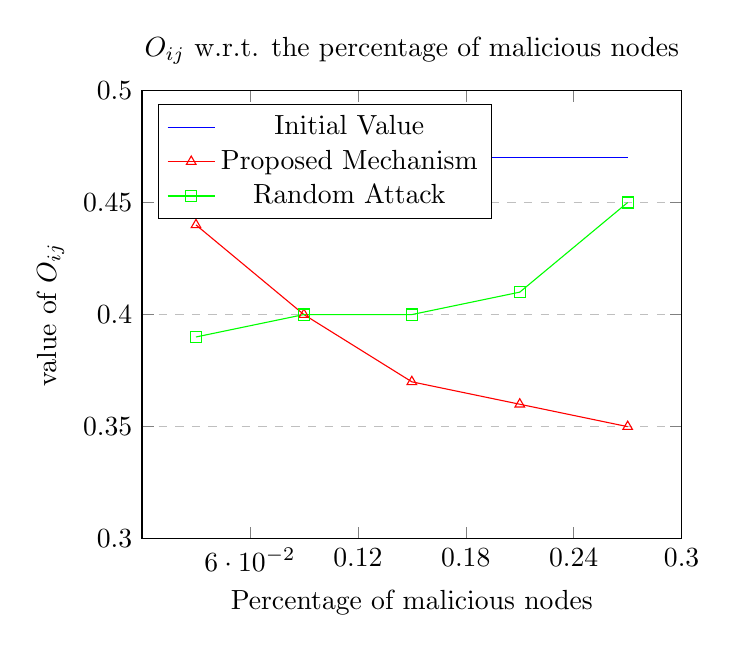
\begin{tikzpicture}
\begin{axis}[
title={$O_{ij}$ w.r.t. the percentage of malicious nodes},
xlabel={Percentage of malicious nodes},
ylabel={value of $O_{ij}$},
xmin=0, xmax=0.3,
ymin=0.3, ymax=0.5,
xtick={0.06,0.12,0.18,0.24,0.3},
ytick={0.3,0.35,0.4,0.45,0.5},
legend pos=north west,
ymajorgrids=true,
grid style=dashed,
]

\addplot[
color=blue,
mark=circle,
]
coordinates {
	(0.03,0.47)(0.09,0.47)(0.15,0.47)(0.21,0.47)(0.27,0.47)
};

\addplot[
color=red,
mark=triangle,
]
coordinates {
	(0.03,0.44)(0.09,0.4)(0.15,0.37)(0.21,0.36)(0.27,0.35)
};

\addplot[
color=green,
mark=square,
]
coordinates {
	(0.03,0.39)(0.09,0.4)(0.15,0.4)(0.21,0.41)(0.27,0.45)
};
\addlegendentry{Initial Value}          
\addlegendentry{Proposed Mechanism}
\addlegendentry{Random Attack}

\end{axis}
\end{tikzpicture}
\caption{The figure shows the value of $O_{ij}$ w.r.t. the percentage of the malicious
	workers. }
\end{figure}

%
\indent From this figure, we can see the proposed attack mechanism performs better than the baseline method overall. When the percentage of the malicious nodes is very low (e.g., 3$\%$), since the malicious nodes are too few to change the final prediction results much, the advantage of the proposed mechanism is small. However, when the percentage of the malicious nodes increases, the advantage of the proposed attack scheme becomes bigger. 
\subsection{Experiment Results for Availability Attack}
In this experiment, we consider the scenarios where the percentage of malicious nodes is low (3\%), and compare the performance of the proposed mechanism with the performance of Rand\_Attack. The measure metric used is the change rate. The experiment is conducted 3 times and we report the average results. The results are shown in table 1.
\begin{table}[h]
\centering
\begin{tabular}{p{2.5cm}|ccc}
	\hline 
	\textbf{Method}& Proposed Mechanism& Random Attack\\
	\hline  
	\textbf{Chage Rate}& 0.302& 0.289\\
	\hline
\end{tabular}
\\
\centering{Table 1}
\end{table}

\indent From this table, we can see the proposed attack mechanism performs better than the baseline method. Since the malicious nodes are too few to change the final prediction results much, the advantage of the proposed mechanism is small. However, we can predict that when the percentage of the malicious nodes increases, the advantage of the proposed attack scheme will become bigger. 

\section{Conclusion}
\label{sec:conclusion}
%
In this paper, we investigate the node embedding in adversarial environments and study the data poisoning attack against link prediction task with the node embedding empowered. In order to find an effective attack strategy for the attacker, we design an intelligent attack mechanism by solving an optimization problem. With the derived optimal attack strategy, the attacker can maximize his attack utility. The experimental results based on real-world datasets demonstrate that the proposed attack mechanism can achieve higher attack utility with very few malicious workers.

% Start of "Sample References" section


% Bibliography
\bibliographystyle{ACM-Reference-Format-Journals}
\bibliography{acmtog-sample-bibfile}
                                % Sample .bib file with references that match those in
                                % the 'Specifications Document (V1.5)' as well containing
                                % 'legacy' bibs and bibs with 'alternate codings'.
                                % Gerry Murray - March 2012



\end{document}
% End of v2-acmtog-sample.tex (March 2012) - Gerry Murray, ACM
